\section{Analyse}

\subsection{Fonctionnement général}

Au lancement du jeu, le joueur peut choisir de lancer une nouvelle partie, une partie existante ou de quitter le jeu. Lors de prochaines versions, d'autres entrées pourraient s'ajouter dans ce menu, comme des options ou la possibilité de réaliser des parties en ligne. Avant de lancer une nouvelle partie, les joueurs doivent d'abord choisir la carte puis leur race, couleur et nom. Une fois en jeu, les joueurs jouent chacun leur tour. À la fin, un écran récapitulatif indique le vainqueur, et les joueurs ont la possibilité de créer une nouvelle partie.

\begin{figure}[h]
  \centering
  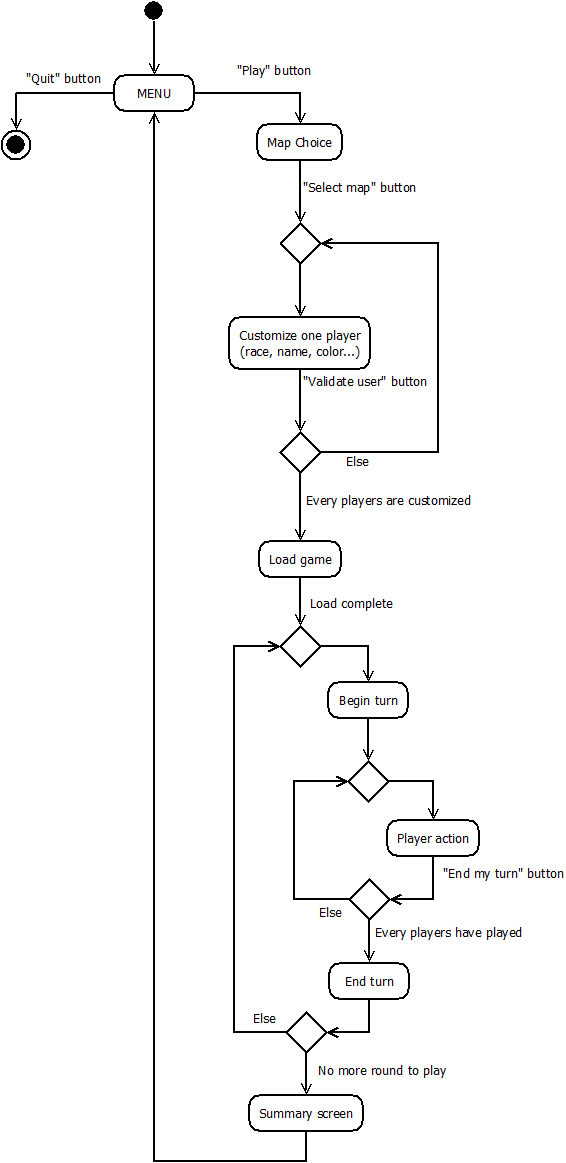
\includegraphics[width=5cm]{schemas/activity.png}
  \caption{Diagramme d'activité}
  \label{activity}
\end{figure}




\subsection{Créer ou charger une partie}

Lorsque le joueur veut lancer un partie, il peut au choix en charger une existante ou en créer une nouvelle. Dans le cas d'une partie existante, la configuration des joueurs, la carte et les unités seront chargés afin de reprendre la partie là où elle en était. Par contre, si le joueur décide de créer une nouvelle partie, alors il devra pouvoir définir tous les paramètres nécessaires.

\begin{figure}[h]
  \centering
  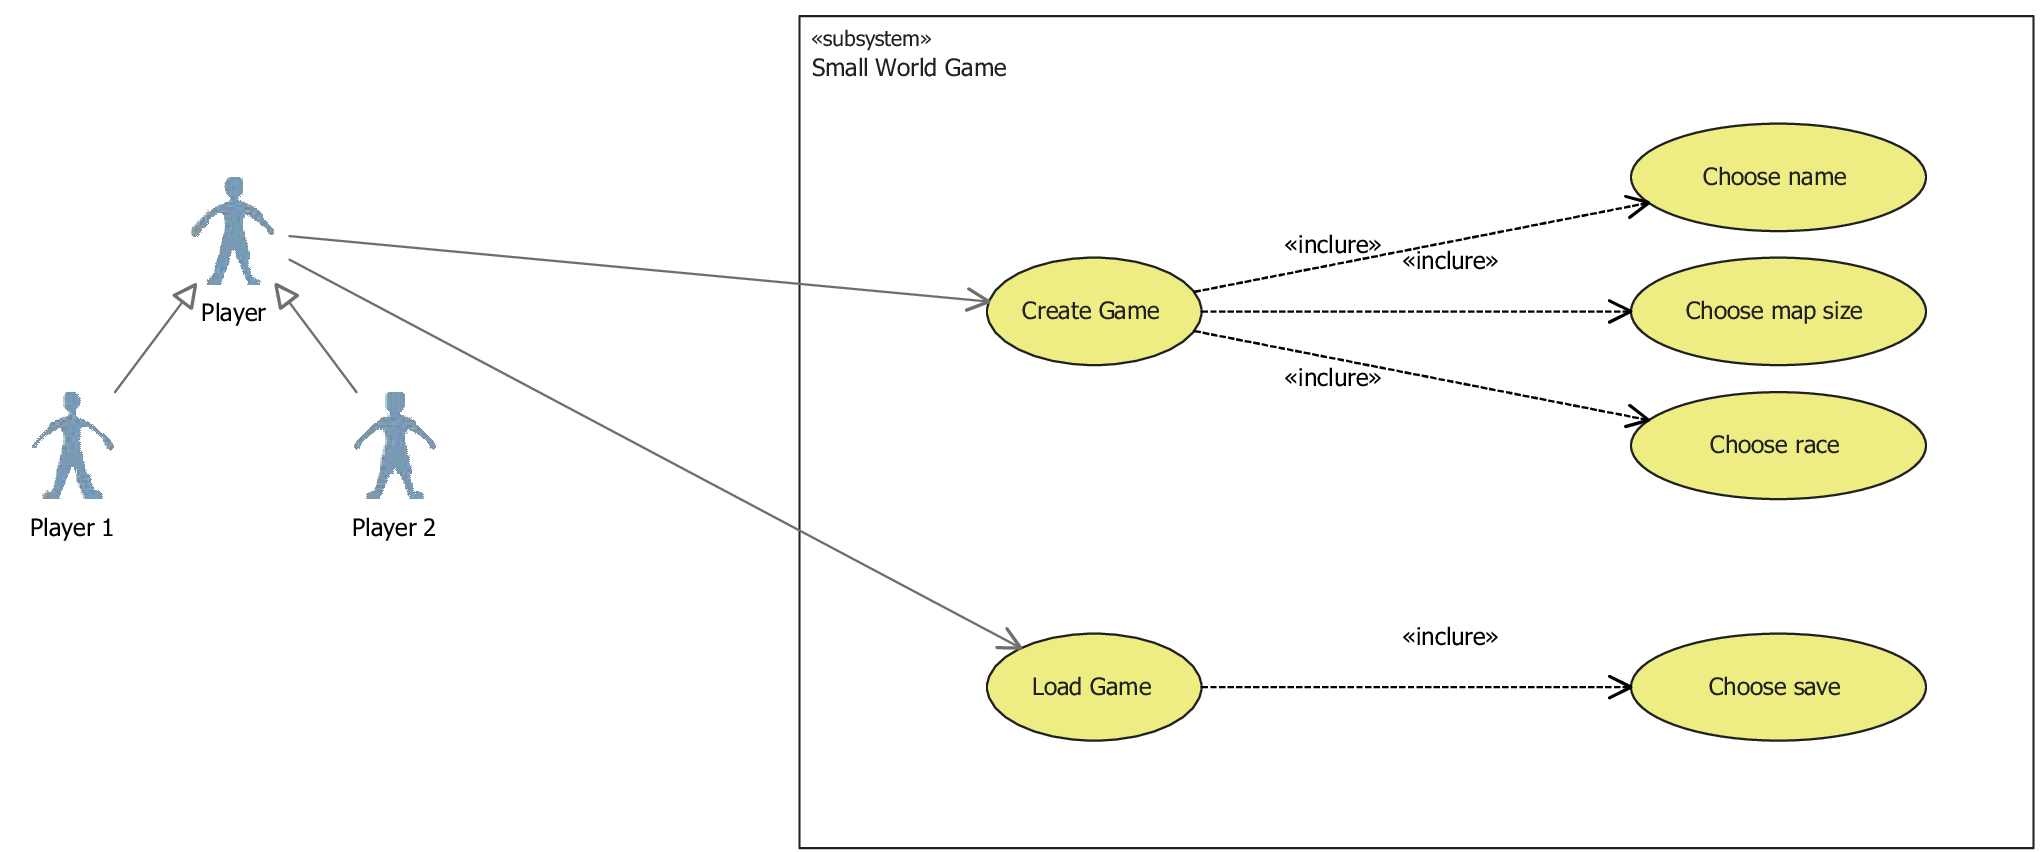
\includegraphics[width=8cm]{schemas/uc_game_creation.png}
  \caption{Diagramme de cas d'utilisation du lancement d'une partie}
  \label{uc_game_creation}
\end{figure}


\subsection{Déroulement d'un tour de jeu}
Lors d'un tour de jeu, le joueur pourra sélectionner ses unités, afin de leur demander de se déplacer ou d'attaquer. Chacune des unités aura 2 points d'action, et pourra donc potentiellement se déplacer et/ou attaquer dans la limite de ses points d'action disponibles.


\subsection{Cycle de vie d'une unité}

Les unités ont un cycle de vie particulier. Grâce aux états définis, nous pouvons imaginer associé un sprite différent en fonction de l'état de cette dernière. Par exemple, les unités dans l'état "Full Life" utiliseront une image d'un personnage en bonne santé, celles dans l'état "Hurt" auront des blessures, et celles dans l'état "Dead" seront représentées par des tombes. Ces états permettent aussi de définir si l'unité peut se déplacer ou pas, etc.

\begin{figure}[!h]
  \centering
  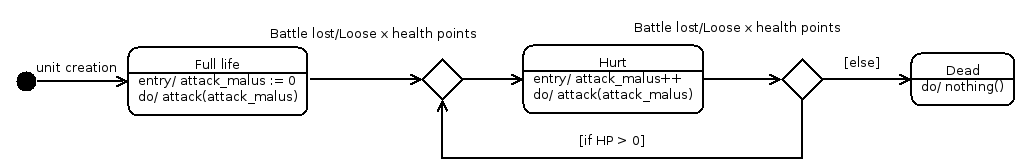
\includegraphics[width=13cm]{schemas/state-diagram.png}
  \caption{Cycle de vie d'une unité}
  \label{state-diagram}
\end{figure}


